\chapter{Conclusions and Future Work}
\label{conclusions_and_future_work}

\section{Summary and Conclusions}

In this upgrade thesis, I have outlined the work I have done so far in my PhD: explored survival analysis in MND, developed a Python library called Fusilli for comparing multimodal machine learning methods, and applied Fusilli to MND data for prognosis prediction.

\subsection{Cox proportional hazards}

Chapter~\ref{cox_proportional_hazards_model} showed the application of a Cox proportional hazards model to multimodal MND data, comprised of baseline clinical features and brain region volumes extracted from structural MRI.
To my knowledge, combining clinical and MRI-derived features in survival analysis for MND has only been done in one paper~\cite{querinSpinalCordMultiparametric2017}, which used spinal cord MRI data and a smaller sample size.
%The main contribution of this chapter was to show that the Cox model could be used to predict prognosis in MND, and that the resulting factors significantly affecting survival are changed when using clinical data, imaging data, or multimodal data.

The multimodal multivariable CPH resulted in two significantly protective factors: the baseline ALSFRS-R score and the bilateral volume of the amygdala, and two significantly harmful factors: the ALS subtype of MND and and larger bilateral lateral ventricle volumes.
The addition of MRI data to clinical information caused a change in the relevance of specific clinical variables within the model, which implied that the brain volumes derived from MRI scans included corresponding information to some clinical features.
In contrast, depending simply on MRI data produced clinically unusual outcomes.
The implications of these findings highlighted the importance of combining imaging data with clinical information for more meaningful survival analysis in MND.

\subsection{Fusilli development}

In Chapter~\ref{fusilli_development}, I showcased Fusilli, my Python library for easy comparison of multimodal data fusion methods, and the steps in its development.
Fusilli is an open-source project, and therefore released for anybody to use in their personal and professional projects.

Key contributions of this chapter were the development of a library that has a catalogue of multimodal data fusion methods that are not limited by their underlying architecture, which is the general limitation of other similar works.
Fusilli was received with interest by the machine learning community, and I have been given feedback from other researchers who have used Fusilli in their projects.

For my future PhD chapters, using Fusilli will greatly speed up my analysis and experimentation.

\subsection{Fusilli for MND prognosis prediction}

My first experimentation with Fusilli for MND prognosis prediction is shown in Chapter~\ref{fusilli_on_mnd}.
The experiment consisted of using baseline clinical data and extracted brain region volumes to predict whether a patient with survive for more or less than 24 months from diagnosis.
Eight multimodal data fusion models, implemented in Fusilli, were compared to each other and to unimodal models.

This experiment resulted in only one of the multimodal models outperforming the unimodal model that used only clinical data.
The validation performance revealed that the models were overfitting, and so further hyperparameter tuning is needed to improve the models to be more generalisable.

In its current form with a small sample size and limited hyperparameter tuning, Fusilli did not show a clear advantage of using multimodal data in MND prognosis prediction, and imaging data may not have been as useful as clinical data in this task.

Further investigation and experimentation are needed to determine the finality of these results.
I hypothesise that with more data, better clinical characterisation, and more fine-grained imaging data, multimodal data fusion will prove to be a useful tool in MND prognosis prediction.

\subsection{Outcomes}

The main outcome of my PhD so far is Fusilli, and I have submitted a paper to the Journal of Open Source Software on the library.

\begin{quote}
Florence Townend, James H Chapman, and James H Cole, (2024). Fusilli: A Python package for multimodal data fusion. Journal of Open Source Software (submitted).
\end{quote}

I have also been second author on a systematic review of explainable machine learning methods in dementia diagnosis:

\begin{quote}
    Sophie A Martin, Florence J Townend, Frederik Barkhof, James H Cole. Interpretable machine learning for dementia: A systematic review. Alzheimer's Dement. 2023; 19: 2135–2149.~\cite{martinInterpretableMachineLearning2023}
\end{quote}

\section{Future Work}

I have split the possible future work sections into roughly three chapters.
Most of the work described relies on the availability of a larger sample size of data from MND cohorts.
My supervisory team and I are liaising with other researchers for access to more data, as well as applying for access to MRI scans from UCLH (University College London Hospitals), which correspond to subjects in ALS Biomarkers Study.

Moreover, I am undertaking a research visit to Charité - Universitätsmedizin Berlin in April and May of 2024, where I will be working on extending Fusilli's capabilities and applying Fusilli to multimodal medical data on mental health and addiction disorders.
%I will be making connections and collaborating with researchers at Charité, and while I am there, I hope to visit MND clinics in Berlin to improve my understanding of other areas of MND clinical research.

\subsection{Applying Fusilli to multimodal medical data: MND and other applications}

The next step in my PhD is to continue applying Fusilli to MND data with larger sample sizes and additional hyperparameter tuning.
I will also apply Fusilli to other multimodal medical datasets to complete the thesis chapter about the library's development.

\subsubsection*{Illustrating Fusilli capabilities with multimodal medical data}

Although Chapter~\ref{fusilli_development} showed the whole development journey of Fusilli, a valuable addition to the narrative would be to show how Fusilli can be used in practice.
I plan to use Fusilli on two multimodal medical datasets.

In terms of feasibility, I already have access to ADNI (Alzheimer's Disease Neuroimaging Initiative) and PPMI (Parkinson's Progression Markers Initiative) data for neurodegenerative diseases, and MIMIC CXR (Medical Information Mart for Intensive Care - Chest X-ray) data for critical care.

Firstly, I will need to preprocess the data by dealing with data missingness in clinical data and running preprocessing pipelines on the imaging data, such as segmentation and registration.
Where appropriate, I will ask for assistance from colleagues who have worked with the data before, and may have already run the preprocessing pipelines.
Next, I will choose a disease-relevant task to apply Fusilli to.
Finally, I will run the Fusilli pipeline on the data, and analyse the results.

\subsubsection*{Extending work on applying Fusilli to MND prognosis prediction}

The next step to extend the work in Chapter~\ref{fusilli_on_mnd} is to include more data from collaborations and the ALS Biomarkers Study, and fine-tune the parameters and architectures of the fusion models, in order to more definitively assess the utility of multimodal data in MND prognosis prediction.
I plan to do this work at the same time as I apply Fusilli to non-MND medical data.

The first step in improving the models would be to examine the preprocessing and feature inclusion of clinical data.
The main additional clinical feature to be added to the analysis would be neurofilament light chain (NfL) measurements from the ALS Biomarkers Study, which are currently too sparse to be used in the models so far, but samples are being analysed to increase the number of measurements available.

Furthermore, collaborators in Jena are running their D50 model on the ALS Biomarkers Study ALSFRS-R data.
Using the D50 will enable the estimation of the ALSFRS-R at the date the MRI was taken, which will allow us to use MRI data from further away from diagnosis alongside the clinical data.
%It will also allow us to investigate the effect on performance when preprocessing the ALSFRS-R data in different ways, such as using the raw scores, the slopes of the raw scores, which have shown promise in a recent paper~\cite{papaizEnsembleimbalancebasedClassificationAmyotrophic2024}, or the D50-estimated ALSFRS-R.
Moreover, we will obtain D50-derived parameters of disease aggressiveness and accumulation, which could be used as added features in the models.

For the imaging data, we will obtain more fine-grained brain measurements from using the \texttt{recon-all} pipeline from FreeSurfer, and use feature selection methods and domain knowledge to decide which measurements to include in the models.

The expected outcomes of this work are more accurate predictions of MND prognosis, and a better understanding of the utility of multimodal data in this application.
Moreover, this work will hopefully reveal a multimodal method that outperforms other methods in the literature, and will be able to be taken forward as the main focus of the next experiments in my PhD.

\subsection{Effect of MRI preprocessing on Fusilli prognosis prediction}

%In Chapter~\ref{literature_review}, it was shown that there are mixed results on the usefulness of neuroimaging in predicting prognosis in MND.
%Many imaging modalities have been studied, such as DTI, fMRI, and structural MRI, and within each of these modalities, there are many preprocessing steps that can be taken to extract features from the images or enhance the information within them for computer-vison tasks.

In this project, I aim to explore the different preprocessing steps that can be taken on structural MRI data to two ends: firstly, to improve the performance of the models, and secondly, to understand which areas of the brain are most important in MND prognosis prediction with machine learning, since Chapter~\ref{literature_review} showed great variability in the results of imaging studies in MND.
A colleague is enhancing clinical MRI quality for ALS Biomarkers Study data via AI techniques, enabling us to use whole-brain images in models and to use preprocessing steps typically challenging with lower-quality clinical scans.

% add methods to this
Some examples of preprocessing steps that could be applied to the MRI data to extract tabular data are
\begin{itemize}
\setlength\itemsep{-0.5em}
    \item Further fine-grained extracted brain measurements from the \texttt{recon-all} pipeline from FreeSurfer.
    \item Cortical thickness measurements through FreeSurfer.
    \item Different atlases for brain region volume extraction.
\end{itemize}

For the images themselves to be included as input into the models, the options for extracting information from the scans could include
\begin{itemize}
\setlength\itemsep{-0.5em}
    \item Texture analysis, which has been previously used in ALS imaging studies~\cite{ishaqueEvaluatingCerebralCorrelates2018, johnsQuantifyingChangesSusceptibility2019}.
    \item Voxel-based morphometry to extract density maps and perform volumetric analysis using SPM (Statistical Parametric Mapping).
    \item White matter hyperintensity segmentation through BaMoS~\cite{fifordAutomatedWhiteMatter2020}
    \item Surface rendering with FreeSurfer to extract maps of the brain surface.
\end{itemize}


We will use Fusilli to compare the performance of the models using various combinations of clinical and processed imaging data.
The quality of the inferences taken from this analysis will depend on the sample size of the data, because imaging is more expensive to process than clinical data.
A larger sample size would offer a clearer understanding of the importance of different brain regions in MND prognosis prediction, and would allow us to use more detailed imaging data in the models.
If the sample size is not large enough, a contingency plan would be to focus on diseases that have more data available, such as Alzheimer's disease or frontotemporal dementia.

The expected outcomes of this project are an understanding of the utility of different preprocessing steps for structural MRI data in MND prognosis prediction, and a better understanding of which areas of the brain are most important in MND prognosis prediction.


\subsection{Final project options}

The final project in this PhD will depend on the availability of data.
We could either add more data modalities to the multimodal models, such as spinal MRI or features derived from radiological reports, or we could investigate the usefulness and sensitivity of the best-performing models on varying definitions of prognosis.

\subsubsection*{Sensitive analysis of Fusilli prognosis prediction on varying prognosis definitions}

Our experimental set-up in Chapter~\ref{fusilli_on_mnd} was to predict whether a patient would survive for more or less than 24 months from diagnosis.
Survival category classification is a common target in MND prognosis prediction~\cite{ongPredictingFunctionalDecline2017,grollemundDevelopmentValidation1year2020, schusterSurvivalPredictionAmyotrophic2017, vanderburghDeepLearningPredictions2017}.
Patients have shown interest in more fine-grained survival predictions, such as actual survival times~\cite{westenengPrognosisPatientsAmyotrophic2018}, but to my knowledge, predicting survival time has not been done in the literature so far.

In this project, we will aim to take the best multimodal model from the previous chapters and apply it to different definitions of prognosis, some of which are based on survival, such as survival time in months, survival categories, and probabilities of survival at different time points.
Other prognosis definitions are focused on functional decline, which could entail predicting future ALSFRS-R scores or progression rates.
Finally, other definitions of prognosis could be the need for and timing of treatment.

Prognosis definitions vary in importance across settings, like survival time in clinical practice and progression rate for trial stratification. While predicting all may be constrained by data availability, we will aim to cover as many as possible.

We expect to find that the performance of the model will change depending on the definition of prognosis.
Through the use of explainability methods, such as guided backpropagation or SHAP values, we will investigate which features are most important in the different definitions of prognosis, and how these features change between the definitions.
%This will give us a better understanding of the utility of multimodal data in MND prognosis prediction, and will allow us to make more informed decisions about which definitions of prognosis to use in future studies.


\subsubsection*{Adding spinal MRI data to Fusilli prognosis prediction}

Features extracted from spinal MRI have been shown to be useful in MND prognosis prediction unimodally~\cite{brancoSpinalCordAtrophy2014, grolezMRICervicalSpinal2018}, and also in combination with clinical data~\cite{querinSpinalCordMultiparametric2017}.

This potential project would focus on adding spinal MRI images or derived features to the multimodal analysis.
The aim would be to investigate the utility of spinal MRI in predicting prognosis with machine learning.
The project would look at its utility in the absence of other data modalities, and also in a multimodal setting: in combination with clinical data, brain MRI data, or both.

The feasibility of this study depends on the availability of spinal MRI.
Some of the subjects in ALS Biomarkers Study have spinal cord MRI data, but it is not complete for all subjects.
Future data collaborations might include spinal MRI data, which would make this project more feasible.

\subsubsection{Adding radiological report derived features to Fusilli prognosis prediction}

Radiological reports are text documents that describe the findings of a radiologist when they have analysed an MRI scan.
Natural language processing (NLP) can be used to extract features from these reports.
%, such as the presence of certain words or phrases, the radiologist's opinion on the scan, and the radiologist's findings.

These derived features could be included as a new data modality into multimodal prognostic models.
Most of the studies using radiological reports for machine learning either focus on mining the reports for prediction labels to train models on~\cite{nowakDevelopmentImagebasedDecision2023}, or trying to predict the reports from the images and vice versa~\cite{panChestRadiologyReport2024, gajbhiyeTranslatingMedicalImage2022}.
Using the reports as a data modality in multimodal models is a novel approach to incorporating the information contained in the reports into the models.

This project would focus on investigating if features extracted from radiological reports add information to multimodal models in Fusilli.
Especially interesting would be to see if the report-derived features improve prognosis prediction when combined with the associated imaging data, or if they are useful on their own.

Although radiological reports should be available for every scan that has been reviewed by a radiologist, the feasibility of this study depends on the availability of the reports in our datasets.
The reports are not available in the cohort from Ospedale San Raffaele, but some subjects in the ALS Biomarkers Study have reports available through the PACS system.

\section{Timeline}

\begin{figure}
    \centering
    \hspace*{-0.1\textwidth}
    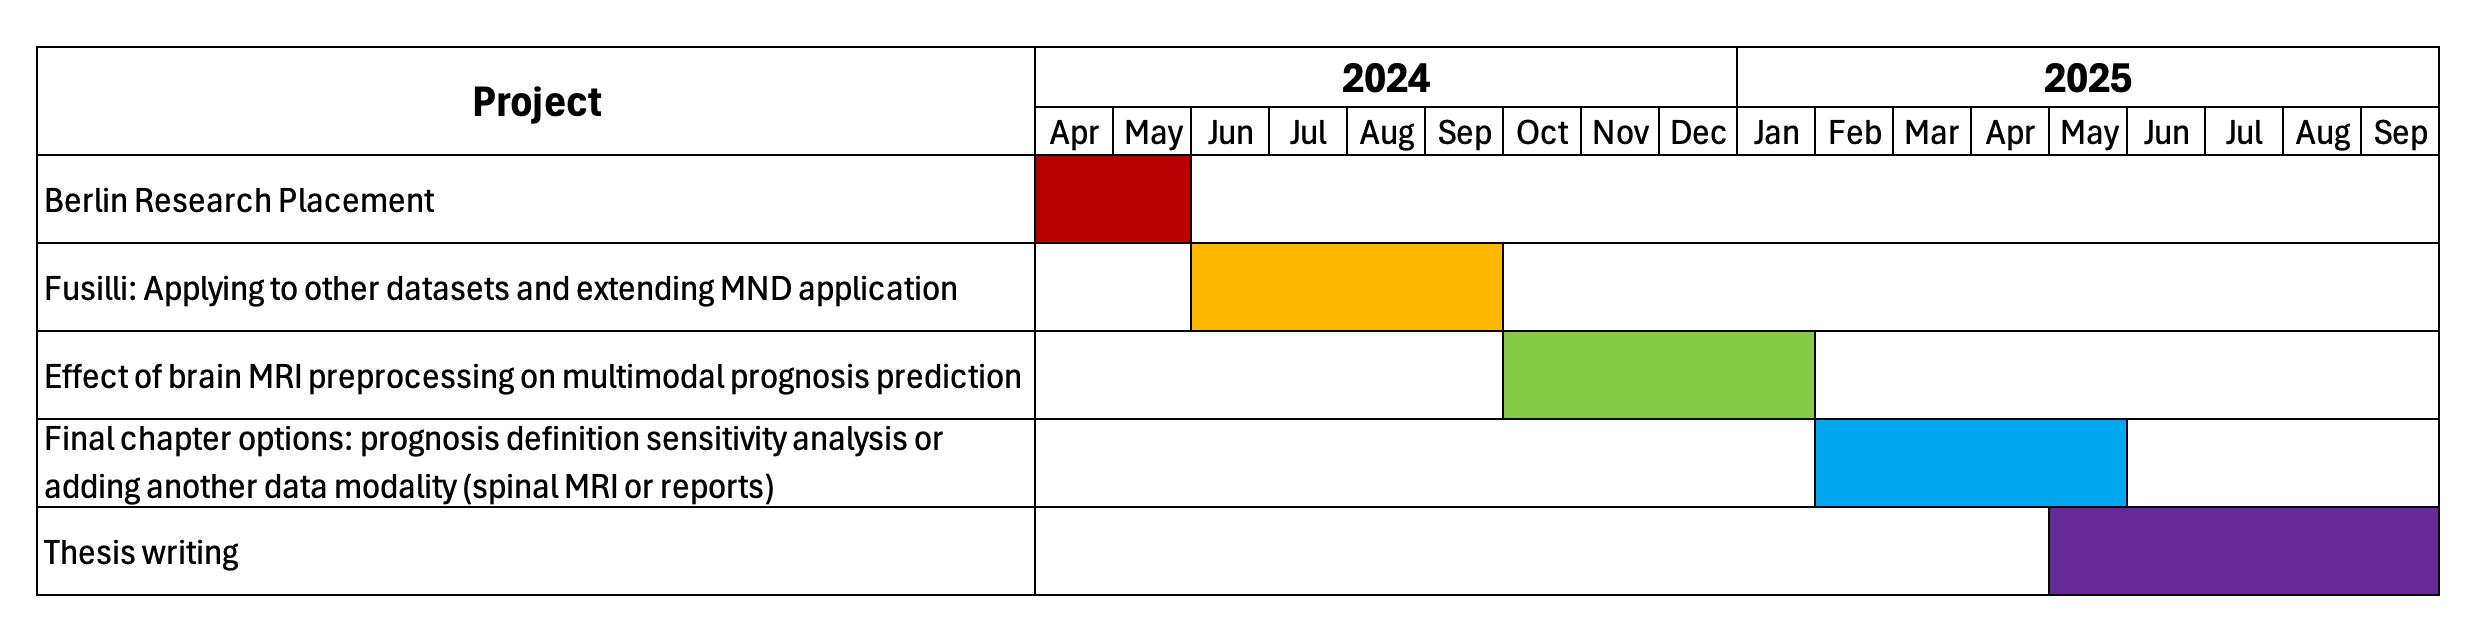
\includegraphics[width=1.2\textwidth]{figures/gantt_chart}
    \caption{Gantt chart showing the timeline for the remaining work in my PhD}
    \label{fig:gantt_chart}
\end{figure}

Figure~\ref{fig:gantt_chart} shows the proposed timeline for the remaining work in my PhD.
I have allotted 5 months to write my thesis.

April and May of 2024 will be spent at Charité - Universitätsmedizin Berlin, and so I have not included any project work in this period in the timeline.
However, I will be working on extending Fusilli's capabilities which will be extensively used in the projects described above.
Moreover, I will be continuing to work on accessing more data from collaborations and the ALS Biomarkers Study.
